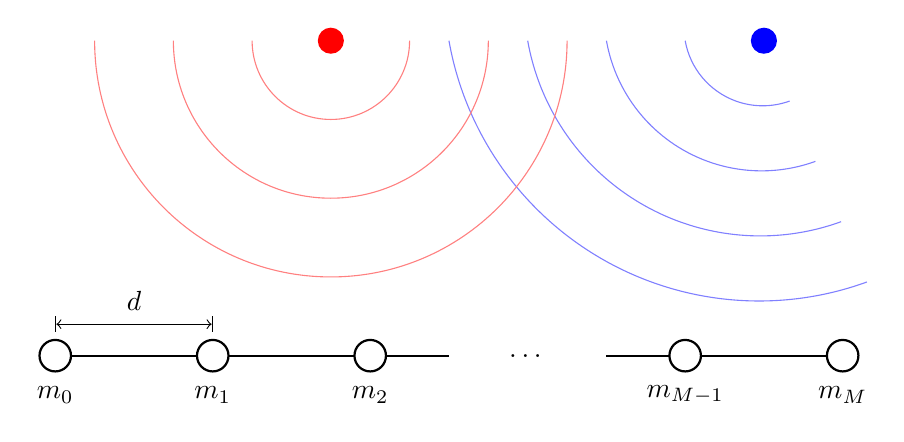
\begin{tikzpicture}
  [mic/.style={shape=circle, black, fill=white, thick, minimum size=4mm}]
  % Setup constants
  \def\miclineoffset{.4}
  \pgfmathsetmacro{\doffset}{\miclineoffset+.3}
  \pgfmathsetmacro{\miclabeloffset}{-.5}
  % Draw the lines on which the microphones will lie
  \draw [thick] (0,0) -- (5,0);
  \draw [thick] (7,0) -- (10,0);
  % Draw the first three mics in the group
  \draw [|<->|] (0,\miclineoffset) -- (2, \miclineoffset);
  \foreach \x in {0, 1, 2} {
    \node at (2*\x, 0) [mic, draw] {};
    \node at (2*\x, \miclabeloffset) {$m_{\x}$};
  }
  % Separator between sets of nodes
  \node at (6, 0) {\ldots};
  % Last few nodes that will be indexed from the end (M)
  \node at (8, 0) [mic, draw] {};
  \node at (8, \miclabeloffset) {$m_{M-1}$};
  \node at (10, 0) [mic, draw] {};
  \node at (10, \miclabeloffset) {$m_{M}$};
  \node at (1, \doffset) [] {$d$};

  % Draw arcs for sound waves
  \node[circle, fill=blue] at (9, 4) {};
  \foreach \rad in {1, 2, 3, 4} {
    \draw[blue!50] (9-\rad, 4) arc [start angle=190, end angle=290, 
    radius=\rad];
  }
  \node[circle, fill=red] at (3.5, 4) {};
  \foreach \rad in {1, 2, 3} {
    \draw[red!50] (3.5-\rad, 4) arc [start angle=180, end angle=360, 
    radius=\rad];
  }
\end{tikzpicture}
